\documentclass{article}

\usepackage{amsmath}
\usepackage{amsthm}
\usepackage{amsfonts}
\usepackage{listings}
\usepackage{xcolor} 
\usepackage{graphicx}
\usepackage{subcaption}
\usepackage[utf8]{inputenc}
\usepackage[russian]{babel}
\usepackage{float}
\usepackage{amssymb}
\usepackage{color}

\DeclareMathOperator*{\argmax}{arg\,max}
\DeclareMathOperator*{\argmin}{arg\,min}

\DeclareMathOperator{\diag}{diag}
\DeclareMathOperator{\tr}{tr}
\DeclareMathOperator{\vect}{vec}
\DeclareMathOperator{\cone}{cone}
\DeclareMathOperator{\dist}{dist}

\newcommand{\R}{\mathbb{R}}
\newcommand{\RV}[1] {\mathbb{R}^{#1}}
\newcommand{\RM}[2] {\mathbb{R}^{#1 \times #2}}
\newcommand{\norm}[1]{\left\lVert#1\right\rVert}

\title{Домашнее задание IV}
\author{Кобылянский А.В. \\ Группа 5381}
\date {}


\definecolor{mygreen}{RGB}{28,172,0} % color values Red, Green, Blue
\definecolor{mylilas}{RGB}{170,55,241}


\begin{document}

    \lstset{language=Python,
        breaklines=true,
        keywordstyle=\color{blue},
        identifierstyle=\color{black},
        stringstyle=\color{mygreen},
        commentstyle=\color{gray},
        showstringspaces=false,%without this there will be a symbol in the places where there is a space
        numbers=left,%
        numberstyle={\tiny \color{black}},% size of the numbers
        numbersep=9pt, % this defines how far the numbers are from the text
        emph=[1]{for, in, while, break},emphstyle=[1]\color{red}, %some words to emphasise
    }

    \pagenumbering{gobble}
    \maketitle
    \newpage
    \pagenumbering{arabic}
    

    \begin{figure}[ht]

        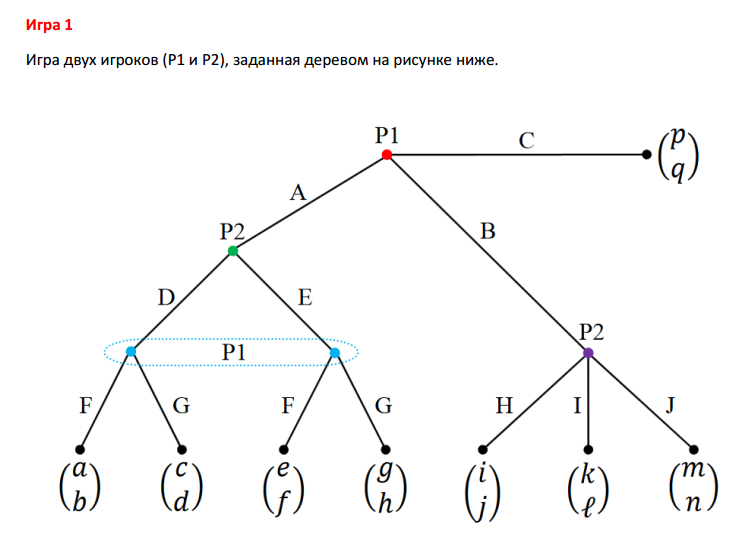
\includegraphics[width=1\linewidth]{imgs/game1.png}

    \end{figure} 
         
    \subsection*{Задача 1}
    Записать \textcolor{red}{Игру 1} в нормальной форме (strategic form), т.е. как биматричную игру: привести матрицы выигрышей (строки соответствуют P1, столбцы соответствуют P2).
    
    \begin{tabular}{l | *{5}{c}r}
           & DH     & DI     &  DJ    & EH     & EI     & EJ \\
        \hline
        AF & (a, b) & (a, b) & (a, b) & (e, f) & (e, f) & (e, f) \\
        AG & (c, d) & (c, d) & (c, d) & (g, h) & (g, h) & (g, h) \\
        BF & (i, j) & (k, l) & (m, n) & (i, j) & (k, l) & (m, n) \\
        BG & (i, j) & (k, l) & (m, n) & (i, j) & (k, l) & (m, n) \\
        CF & (p, q) & (p, q) & (p, q) & (p, q) & (p, q) & (p, q) \\
        CG & (p, q) & (p, q) & (p, q) & (p, q) & (p, q) & (p, q) \\
    \end{tabular}
    
    \subsection*{Задача 2}
    Записать \textcolor{red}{Игру 1} в секвенциальной форме (strategic form); привести матрицы выигрышей (строки соответствуют P1, столбцы соответствуют P2).
     \begin{tabular}{  l| *{5}{c}  r}
           & $\varnothing$ & D  &  E     & H      & I      & J \\
        \hline
$\varnothing$ & 0      & 0      & 0      & 0      & 0      & 0 \\
            A & 0      & 0      & 0      & 0      & 0      & 0  \\
            B & 0      & 0      & 0      & (i, j) & (k, l) & (m, n) \\
            C & (p, q) & 0      & 0      & 0      & 0      & 0  \\
           AF & 0      & (a, b) & (e, f) & 0      & 0      & 0\\
           AG & 0      & (c, d) & (g, h) & 0      & 0      & 0 \\
    \end{tabular}
    
    
    \subsection*{Задача 3}
    Пусть \textcolor{red}{Игра 1} является игрой с нулевой суммой: $a = -b, c = -d,$ и т.д., а выигрыши игрока P1 равны:
    \bigbreak
    \begin{tabular}{| l *{6}{|c} | r |}
        \hline
        a  & c   &  e & g  & i & k & m & p \\  
        \hline
        10 & -11 & -8 & 14 & 1 & 2 & 3 & 0 \\
        \hline        
    \end{tabular}
    \bigbreak
    
    Найти равновесные смешанные стратегии, а так же цену игры с помощью:
    
    1. Онлайн сервиса для нормальной формы игры.
     \bigbreak
    Результат работы программы:\\
    The matrix is\\
    10 10 10 -8 -8 -8\\
    -11 -11 -11 14 14 14\\
    1 2 3 1 2 3\\
    1 2 3 1 2 3\\
    0 0 0 0 0 0\\
    0 0 0 0 0 0\\
    The value is 1.2093.\\
    An optimal strategy for Player I is:\\
    (0.5814,0.4186,0,0,0,0)\\
    An optimal strategy for Player II is:\\
    (0.51163,0,0,0.48837,0,0)\\
    
    2. Решения пары задач линейного программирования для игры в секвенциальной форме (используя библиотеку cvxopt).
    
    \begin{figure}[ht]

        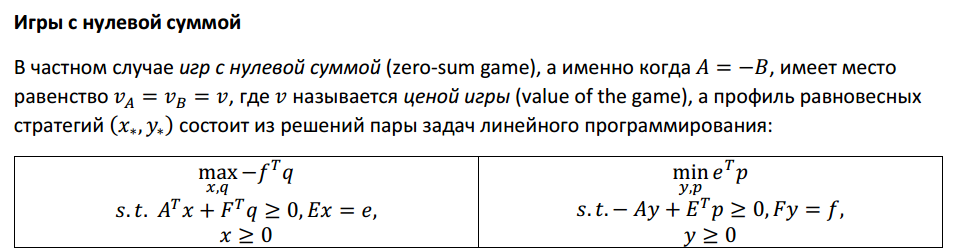
\includegraphics[width=1\linewidth]{imgs/task3_theory.png}

    \end{figure} 
    
    Если вектор $x$ соответствует последовательностям $[\varnothing, A, B, C, AF, AG]$, а вектор $y$ последовательностям $[\varnothing, D, E, H, I, J]$, то 
    
    \begin{equation*}
        A = \left(
        \begin{matrix}
            0 & 0 & 0 & 0 & 0 & 0\\
            0 & 0 & 0 & 0 & 0 & 0\\
            0 & 0 & 0 & 1 & 2 & 3 \\
            0 & 0 & 0 & 0 & 0 & 0 \\
            0 & 10 & -8 & 0 & 0 & 0 \\
            0 & -11 & 14 & 0 & 0 & 0
        \end{matrix}
        \right)
    \end{equation*}
    
    \begin{equation*}
        \begin{cases} 
            x_0 = 1 \\ 
            x_1 + x_2 + x_3 = x_0\\
            x_4 + x_5 = x_1
        \end{cases} \Rightarrow
        E = \left(
        \begin{matrix}
            1 & 0 & 0 & 0 & 0 & 0\\
            -1 & 1 & 1 & 1 & 0 & 0\\
            0 & -1 & 0 & 0 & 1 & 1 \\
        \end{matrix}
        \right),
        e = \left(
        \begin{matrix}
            1\\
            0\\
            0
        \end{matrix}
        \right)
    \end{equation*}
    
    \begin{equation*}
        \begin{cases} 
            y_0 = 1 \\ 
            y_1 + y_2 = y_0\\
            y_3 + y_4 + y_5 = y_0
        \end{cases} \Rightarrow
        F = \left(
        \begin{matrix}
            1 & 0 & 0 & 0 & 0 & 0\\
            -1 & 1 & 1 & 0 & 0 & 0\\
            -1 & 0 & 0 & 1 & 1 & 1 \\
        \end{matrix}
        \right),
        f = \left(
        \begin{matrix}
            1\\
            0\\
            0
        \end{matrix}
        \right)
    \end{equation*}
    \bigbreak
    
    Код решения:
    \lstinputlisting{Source/task3.py} 
    
    \newpage
    Цена игры такая же, как и в первом пункте: $1.2093$.
    
    Ниже приведены равновесные смешанные стратегии полученные в первом пункте \textcolor{red}{(красным)} и втором пункте \textcolor{green}{(зеленым)}. Они тоже практически одинаковы, кроме ребер $H, I, J$.
    \begin{figure}[ht]

        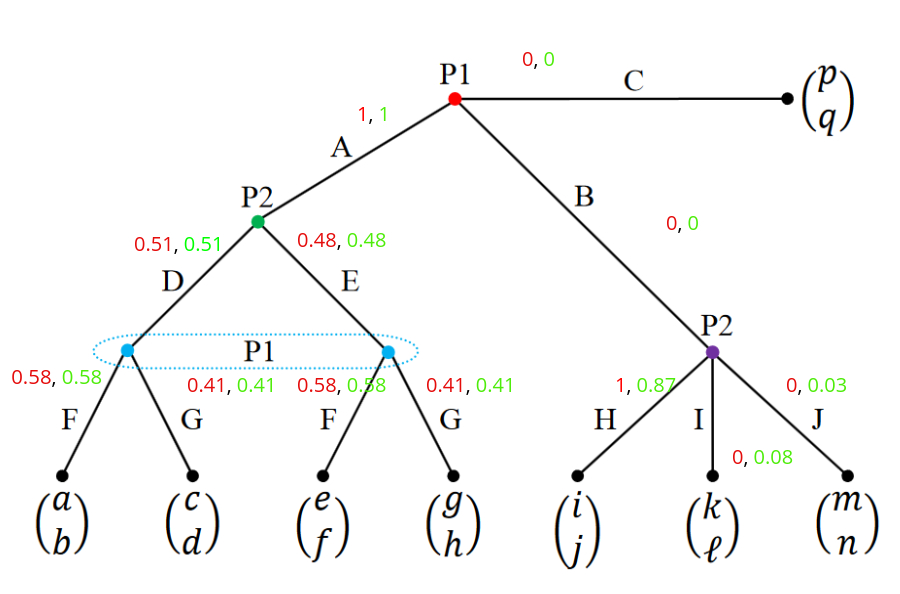
\includegraphics[width=1\linewidth]{imgs/task3_res.jpg}

    \end{figure}     
\end{document}

    


    
    
